%%%%%%%%%%%%%%%%%%%%%%%%%%%%%%%%%%%%%%%%%
% University/School Laboratory Report
% LaTeX Template
% Version 3.1 (25/3/14)
%
% This template has been downloaded from:
% http://www.LaTeXTemplates.com
%
% Original author:
% Linux and Unix Users Group at Virginia Tech Wiki 
% (https://vtluug.org/wiki/Example_LaTeX_chem_lab_report)
%
% License:
% CC BY-NC-SA 3.0 (http://creativecommons.org/licenses/by-nc-sa/3.0/)
%
%%%%%%%%%%%%%%%%%%%%%%%%%%%%%%%%%%%%%%%%%

%----------------------------------------------------------------------------------------
%	PACKAGES AND DOCUMENT CONFIGURATIONS
%----------------------------------------------------------------------------------------

\documentclass{article}

\usepackage{graphicx} % Required for the inclusion of images
\usepackage{amsmath} % Required for some math elements 
\usepackage{cite}
\usepackage{subcaption} %Required to group figures
%\usepackage{float}

\setlength\parindent{0pt} % Removes all indentation from paragraphs

%\usepackage{times} % Uncomment to use the Times New Roman font

%----------------------------------------------------------------------------------------
%	DOCUMENT INFORMATION
%----------------------------------------------------------------------------------------

\title{Lab 5\\ Baseband PAM\\ EE 445S} % Title

\author{Enoc Balderas\\
        \and
        Daniel Diamont\\} % Author name

\date{\today} % Date for the report

\begin{document}

\maketitle % Insert the title, author and date

\begin{center}
\begin{tabular}{l r}
Date Performed: & March 1, 2019 \\ % Date the experiment was performed
Instructor: & Professor Evans % Instructor/supervisor
\end{tabular}
\end{center}

% If you wish to include an abstract, uncomment the lines below
% \begin{abstract}
% Abstract text
% \end{abstract}

%----------------------------------------------------------------------------------------
%	SECTION 1
%----------------------------------------------------------------------------------------

\section{Introduction}

In this lab, we investigated aspects of pulse amplitude modulation (PAM) for baseband transmission and reception. The lab was split up into the following three parts: pulse shaping, symbol clock recovery, and demodulation.

\subsection{Pulse Shaping}
Pulse shaping refers in this case to applying a band-limited pulse to an impulse train of symbol amplitudes before sending the signal to the DAC. In this lab, we explored the effects of using differently parametrized raised cosine pulses on the time domain representation of the signal, as well as the effects on quantization given differences in intersymbol interference.

\subsection{Symbol Clock Recovery (SCR)}
The goal of SCR is for the receiver to re-generate the clock signal that the transmitter used to transmit the data in order for the receiver to properly sample the incoming transmission. The only necessary knowledge that the receiver needs in this case is to know the bandwidth of symbol pulse shape. Since the pulse is designed to minimize inter symbol interference, the receiver can expect the maximum frequency of the transmission to be $ \frac{f_{sym}}{2}. $ Using a band-pass filter, we can recover a cosine with frequency $ \frac{f_{sym}}{2}. $ Since we want $ f_{sym}, $ we can square the signal in the time domain (convolution with itself in the frequency domain) to obtain a spectrum with a DC component and frequencies at $ - f_{sym} $ and $ f_{sym}.$ Lastly, we add another bandpass filter to remove the DC component and any high frequency noise, and this recovers the clock used by the transmitter.

\subsection{Demodulation}
Demodulation in this case refers to recovering a baseband signal that has been modulated with a carrier wave. Part of classic reconstruction, the process is to multiply the signal once again at the receiver by the carrier wave. Since, modulating by the carrier wave twice, i.e., once at the transmitter and once at the receiver, amounts to running the signal through a squaring block, we get a copy of the signal at baseband, and a copy of the signal at plus/minus twice the carrier frequency. Then, we run this result through a low-pass filter to get rid of the high frequency copies of the signal, and we obtain the initial signal at baseband.

%----------------------------------------------------------------------------------------
%	SECTION 2
%----------------------------------------------------------------------------------------

\section{Methods}

\subsection{Pulse Shaping}
First, we created a sequence of 200 random BPSK symbols, and we designed the two raised cosine filters used to pulse shape the sequence to prepare it for transmission. We upsambled the sequence and convolved with the pulse shapes in order to interpolate between the original symbol amplitudes. We used the 'eyediagram' command in MATLAB to explore the impact of each pulse shape on intersymbol interference (ISI). We found that the raised cosine with $ \beta = 1 $ perfomed better in terms of ISI in comparison to the raised cosine with $ \beta = 0.125. $
\linebreak
Specifically, since the raised cosine pulse shape with $ \beta = 1 $ has most of its power in the time domain inside of of the symbol period, then it follows that using the raised cosine to shape successive symbol amplitudes causes less inter symbol interference (ISI). In contrast, using a raised cosine with $ \beta = 0.125, $ which has more power leakage across time with respect to the previous example, then it follows that there will be more inter symbol interference. We can see the difference in ISI by comparing the eye diagrams in Figure 3 and Figure 4. It is clear that we would be able correctly quantize with a higher probability data using a raised cosine with $ \beta = 1 $ as opposed to data using raised cosine with $ \beta = 0.125. $

\subsection{Symbol Clock Recovery}
First, we created two IIR bandpass filters: one to retrieve a cosine at $ \frac{f_{sym}}{2} $ from the original signal, and one to remove the DC component of the squared cosine with a frequency at $ f_{sym}. $ We were able to easily recover the clock frequency used to carry the symbol amplitudes.

\subsection{Demodulation}
As discussed in the introduction, the demodulation process, when assuming a perfect channel, is to multiply again by the carrier wave, and then to run the signal by a low-pass filter to obtain the data at baseband without the high frequency copies.

%----------------------------------------------------------------------------------------
%	SECTION 3
%----------------------------------------------------------------------------------------

\section{Results}

\subsection{Pulse Shaping}

\begin{figure}[h]
  \begin{center}
    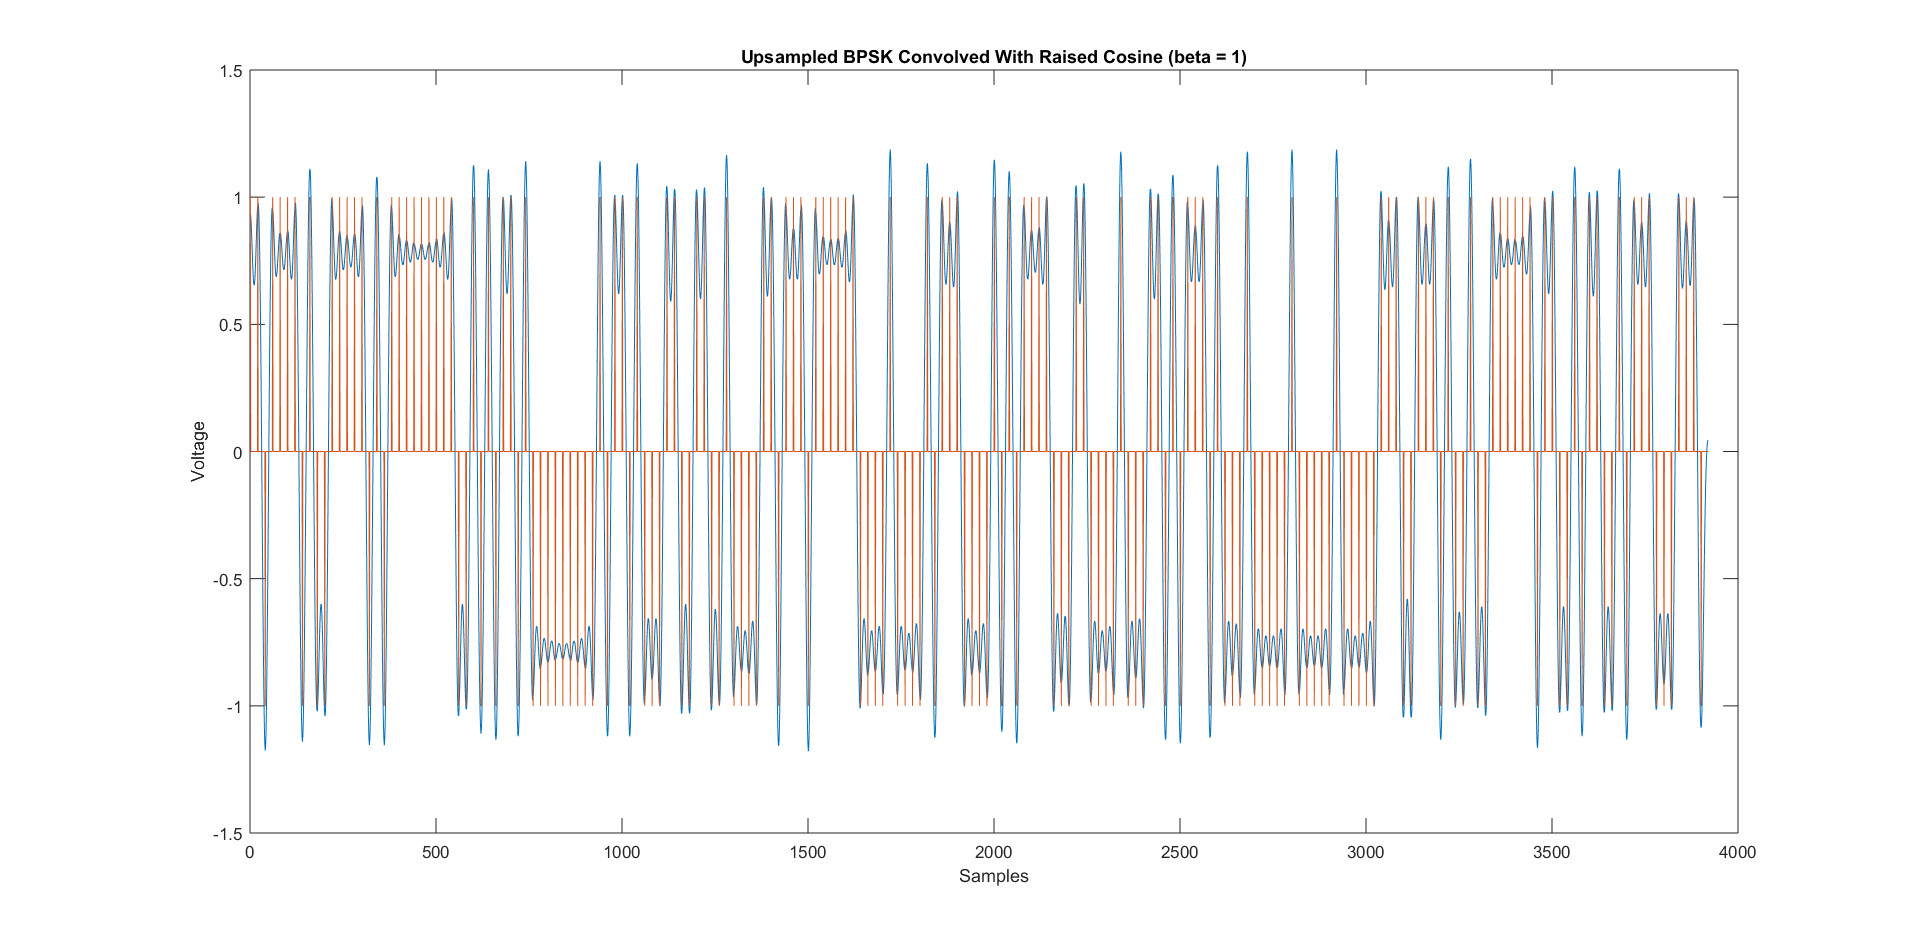
\includegraphics[width=0.65\textwidth]{img/upsampled_bpsk_raised_cosine_beta_1.png}
    \caption{Pulse shaped BPSK $\beta = 1$.}
  \end{center}
\end{figure}

\begin{figure}[h]
  \begin{center}
    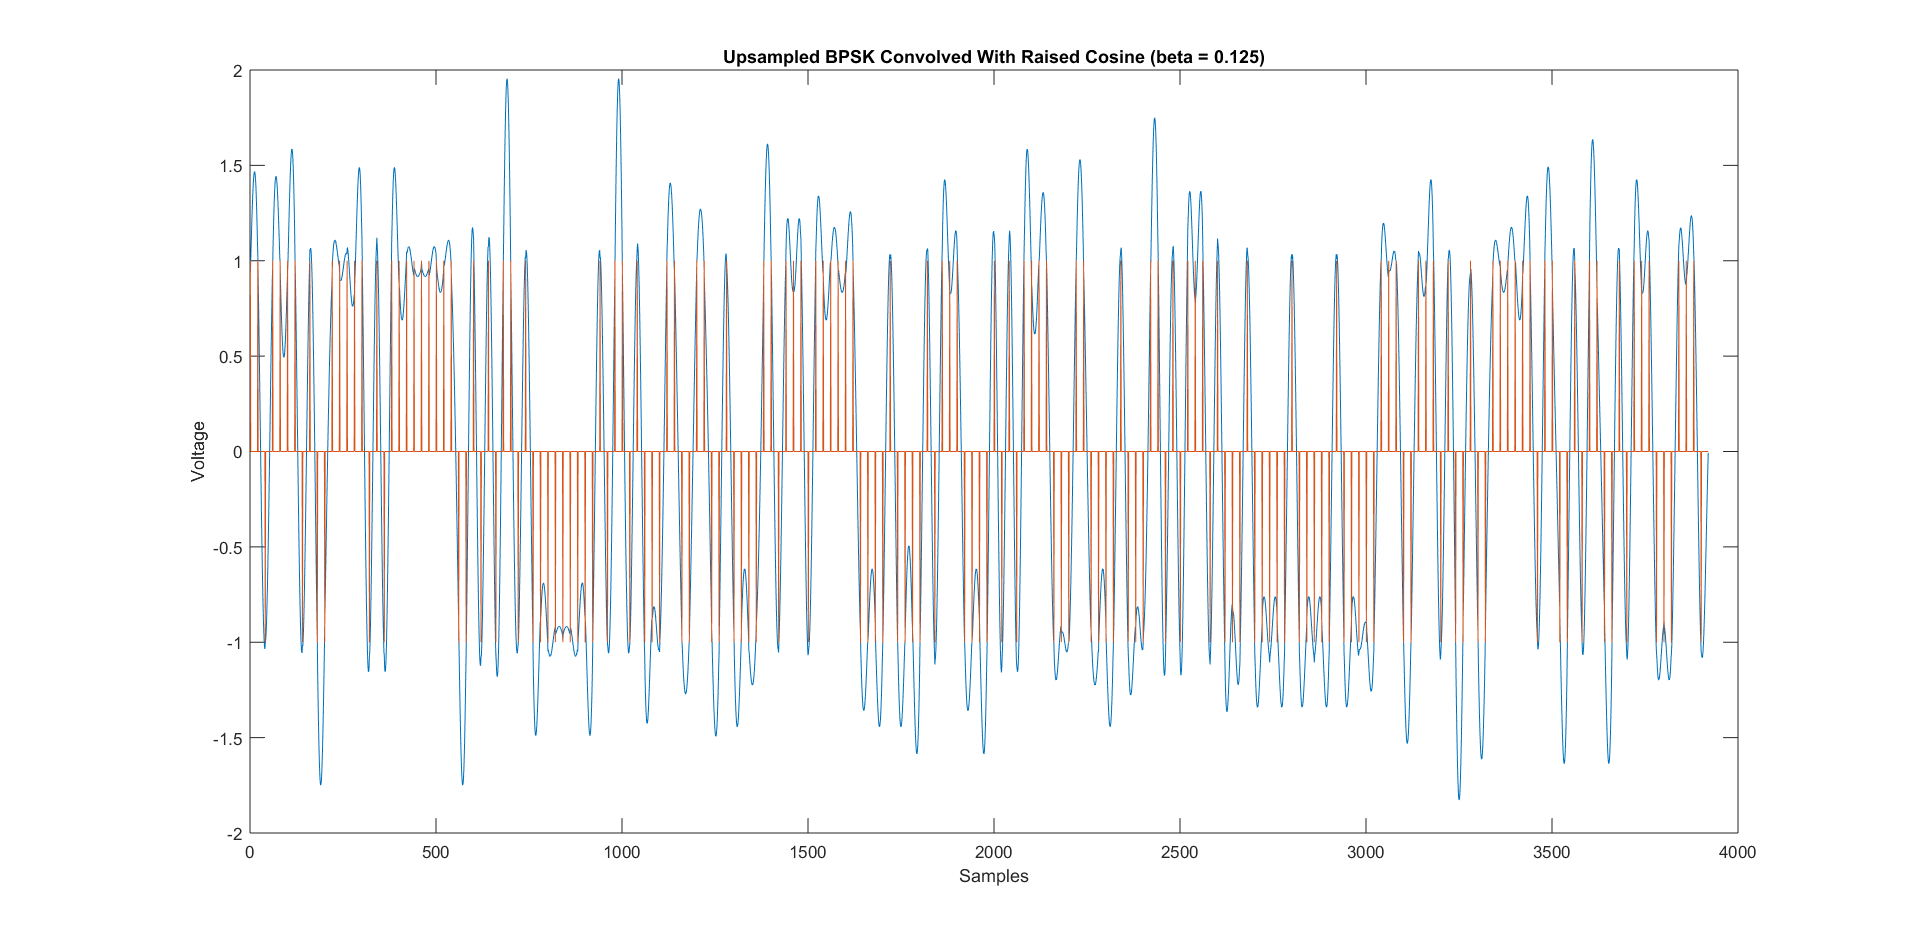
\includegraphics[width=0.65\textwidth]{img/upsampled_bpsk_raised_cosine_beta_125.png}
    \caption{Pulse shaped BPSK $\beta = 0.125$.}
  \end{center}
\end{figure}

\begin{figure}[h]
  \begin{center}
    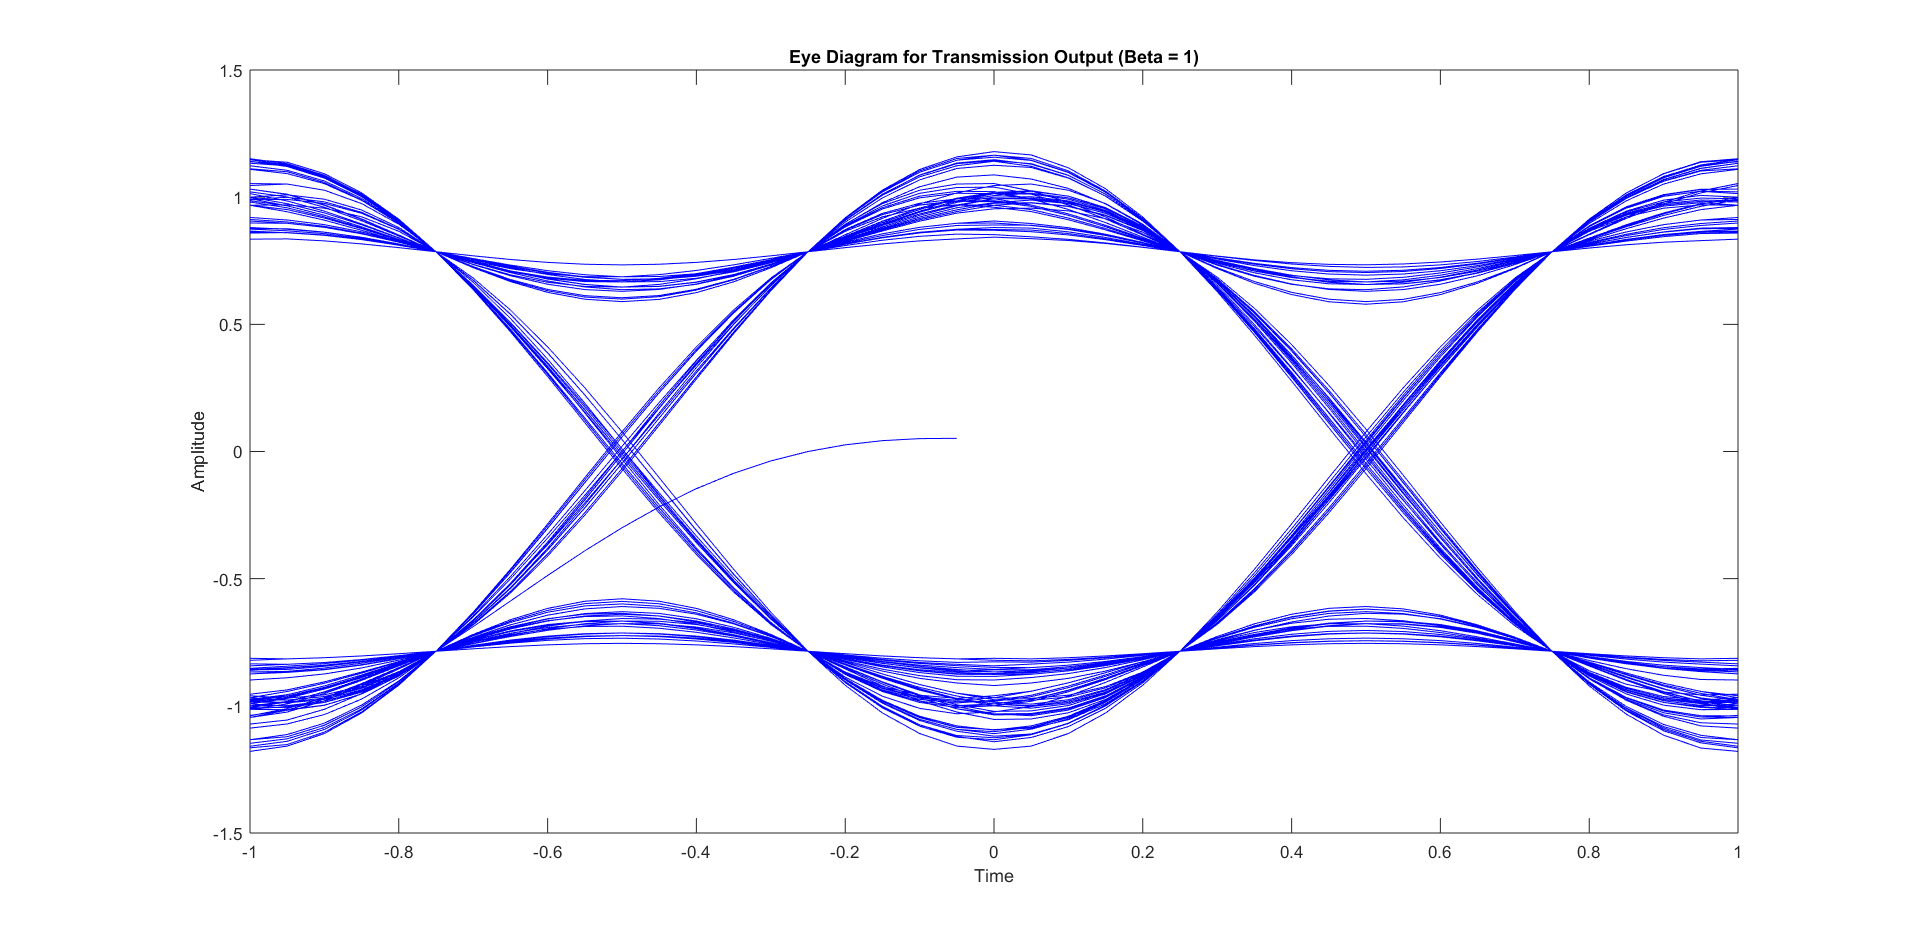
\includegraphics[width=0.65\textwidth]{img/eye_diagram_beta_1.png}
    \caption{Eye Diagram $\beta = 1$}
  \end{center}
\end{figure}

\begin{figure}[h]
  \begin{center}
    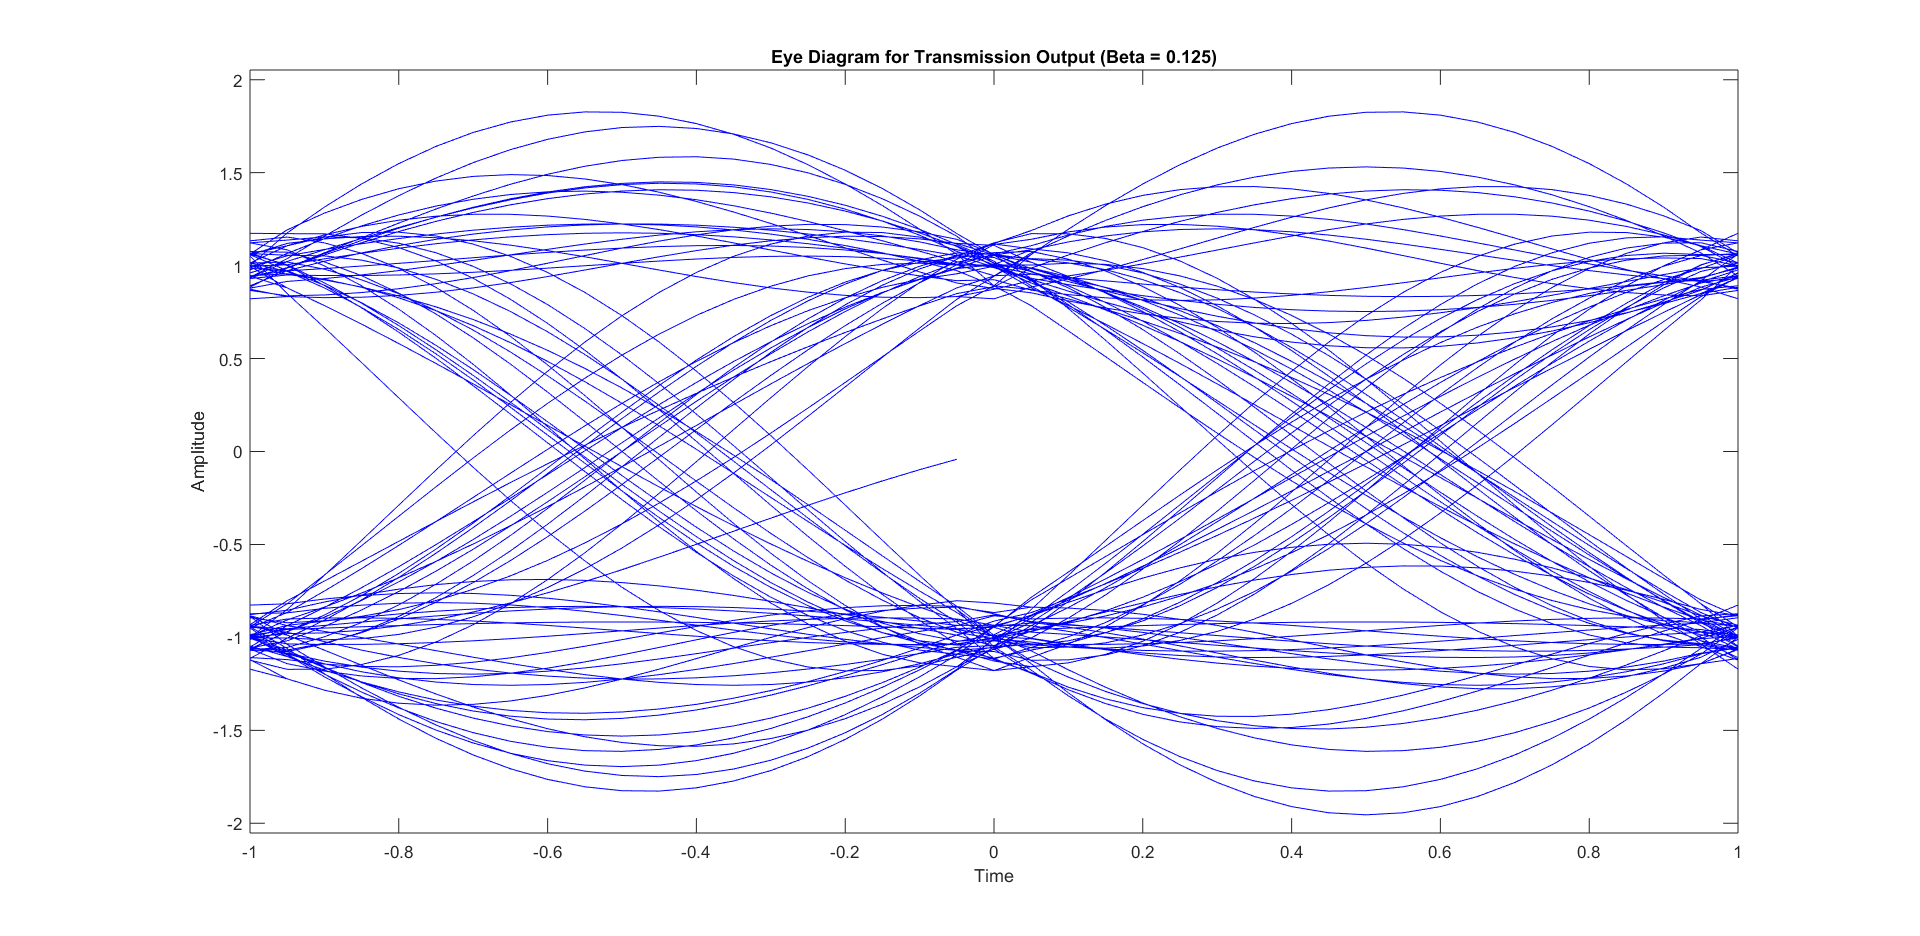
\includegraphics[width=0.65\textwidth]{img/eye_diagram_beta_125.png}
    \caption{Eye Diagram $\beta = 0.125$}
  \end{center}
\end{figure}

\begin{figure}[h]
  \begin{center}
      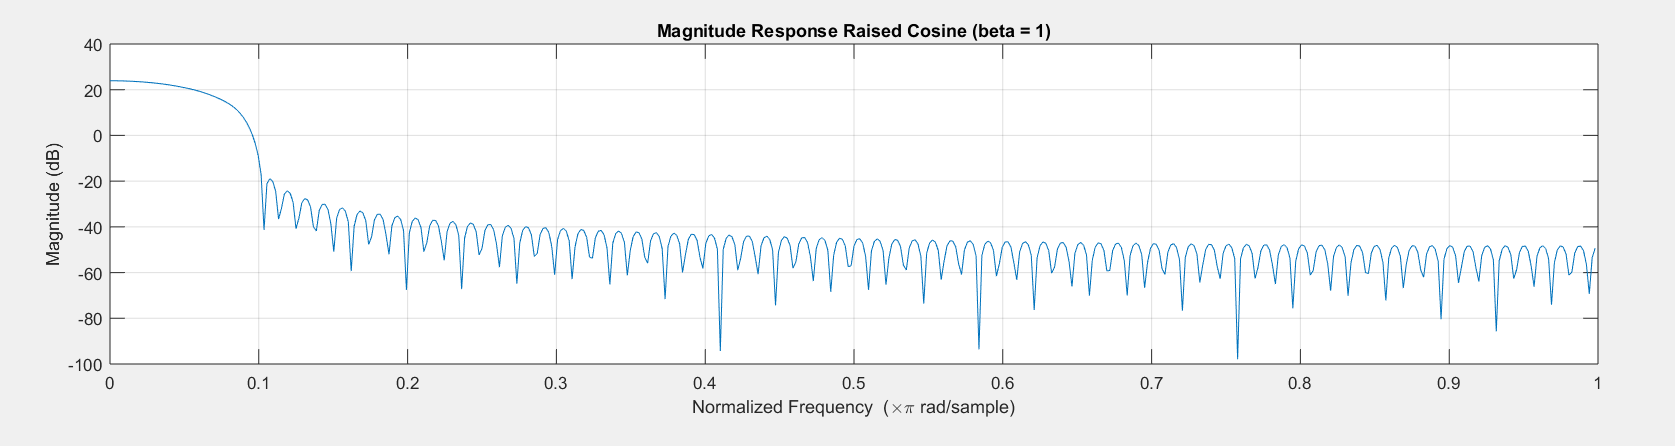
\includegraphics[width=\linewidth]{img/magnitude_response_beta_1.png}
      \caption{Magnitude Response $\beta = 1$}
  \end{center}
\end{figure}

\begin{figure}[h]
  \begin{center}
      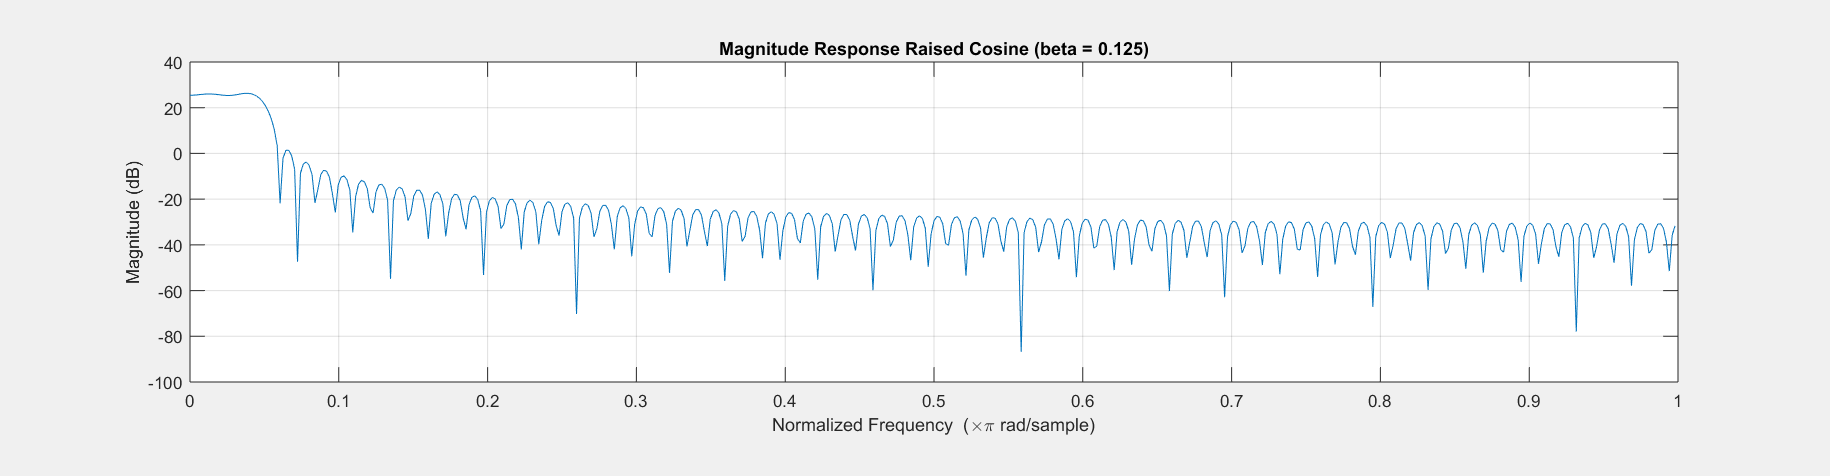
\includegraphics[width=\linewidth]{img/magnitude_response_beta_125.png}
      \caption{Magnitude Response $\beta = 0.125$}
  \end{center}
\end{figure}

\begin{figure}[h]
  \begin{center}
      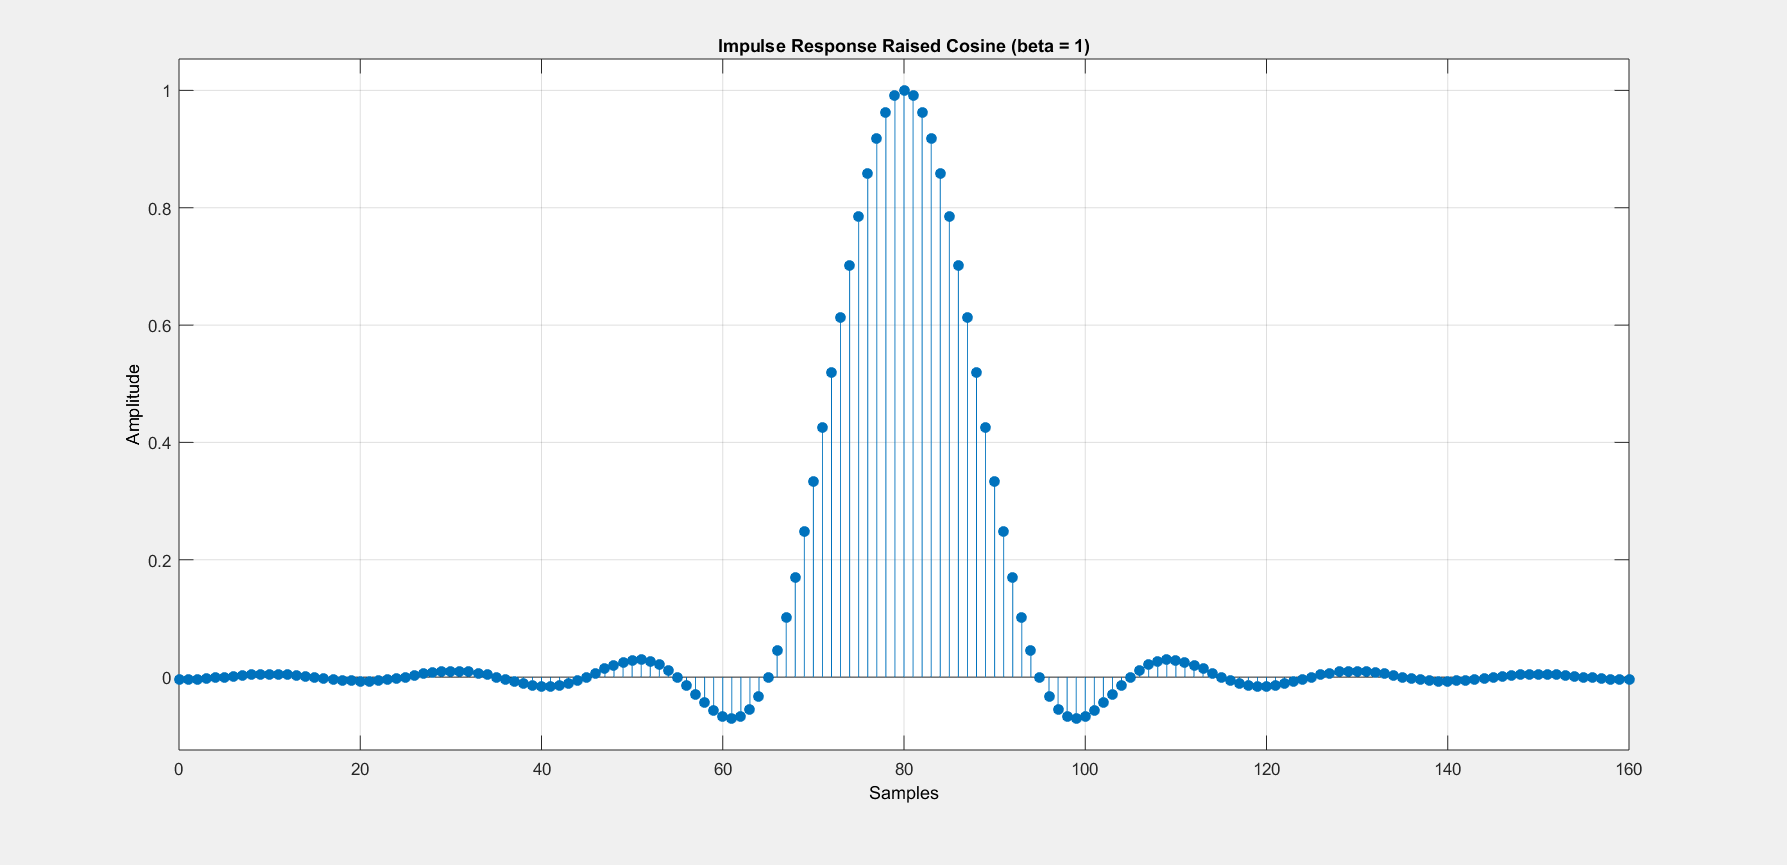
\includegraphics[width=\linewidth]{img/impulse_response_beta_1.png}
      \caption{Time Response $\beta = 1$}
  \end{center}
\end{figure}

\begin{figure}[h]
  \begin{center}
      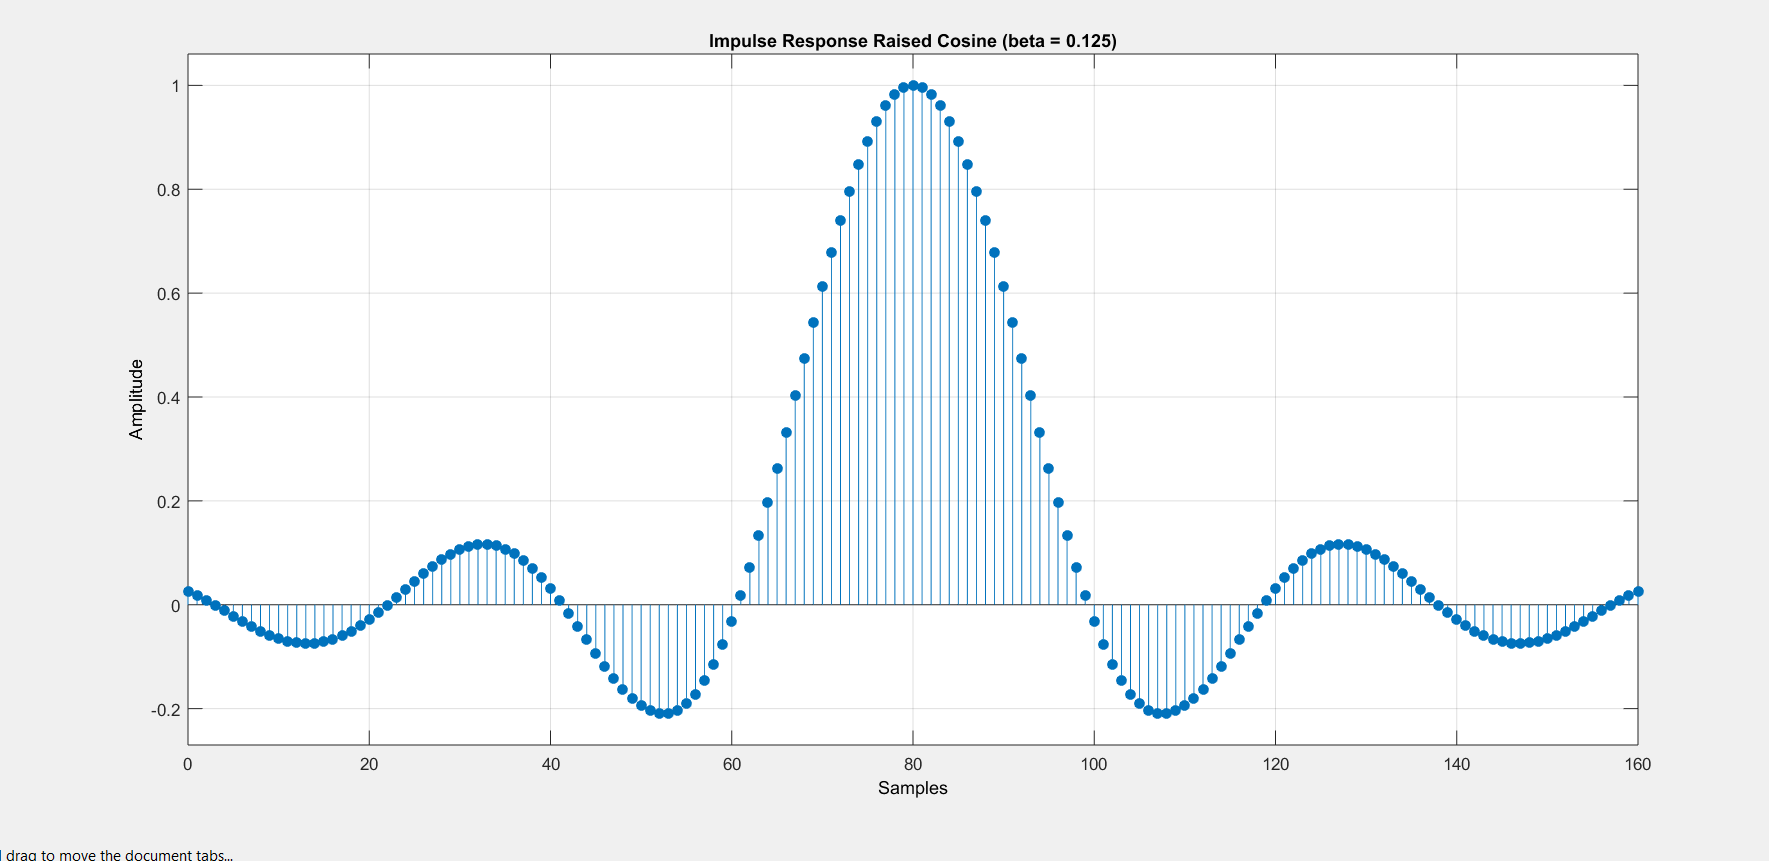
\includegraphics[width=\linewidth]{img/impulse_response_beta_125.png}
      \caption{Time Response $\beta = 0.125$}
  \end{center}
\end{figure}

\clearpage
\pagebreak
\begin{enumerate}
  \begin{item}
  Explain the major differences between the two filters with respect to their
    A) Magnitude responses 
    B) Impulse responses

  \textbf{Answer:}
    A) The main difference between the magnitude response is that the $\beta = 0.125$ filter has
    a much lower bandwidth than the $\beta = 1$ filter.\\

    B) The main difference between the impulse response is that the $\beta = 0.125$ filter
    side lobes decay at a slower rate than the $\beta = 1$ filter side lobes.
  \end{item}

  \begin{item}
    What is the width of the impulse response for the $\beta = 0.125$ case? 

  \textbf{Answer:}
    From the pulse shape samples for the $\beta = 0.125$ filter it looks like there are significant impulses at all 160 samples.
  \end{item}

  \begin{item}
    How would you obtain this number theoretically? (Hint: Look at the fsym and truncation limit you set)

  \textbf{Answer:}
    We could evaluate the pulse shape with the specific parameters that we used in the lab and truncate after it falls below a specific threshold.
  \end{item}

\end{enumerate}

\begin{figure}[h]
  \begin{center}

    \begin{subfigure}[b]{\linewidth}
			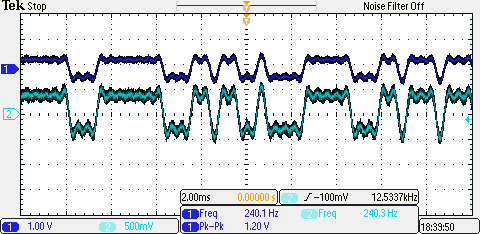
\includegraphics[width=\textwidth]{img/DSK_implementation_beta_1.png}
      \caption{Time Response $\beta = 1$}
    \end{subfigure}

    \begin{subfigure}[b]{\linewidth}
			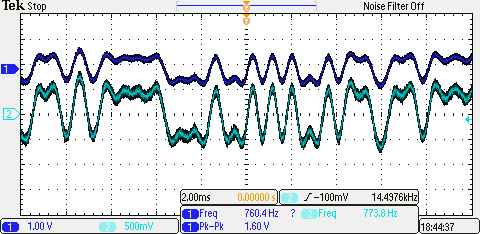
\includegraphics[width=\textwidth]{img/DSK_implementation_beta_125.png}
      \caption{Time Response $\beta = 0.125$}
    \end{subfigure}

  \end{center}
\end{figure}

\clearpage
\pagebreak
\subsection{Symbol Clock Recovery}

\textbf{Prefilter:}

\begin{center}
\begin{tabular}{c|c}
b0	&	 1				\\ \hline
b1	&  0				\\ \hline
b2	& -1				\\ \hline
-a1	&	 1.96004	\\ \hline
-a2	&	-0.984414
\end{tabular}
\end{center}

\textbf{Bandpass:}

\begin{center}
\begin{tabular}{c|c}
b0	&	 1				\\ \hline
b1	&  0				\\ \hline
b2	& -1				\\ \hline
-a1	&	 1.87293\\ \hline
-a2	&	-0.969067
\end{tabular}
\end{center}

\begin{figure}[h]
  \begin{center}
    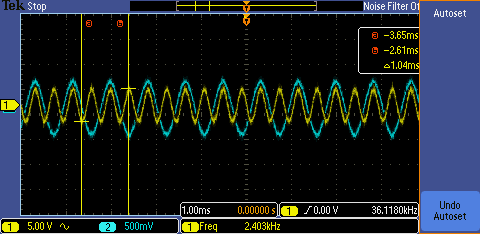
\includegraphics[width=0.65\textwidth]{img/dotting_sequence_SCR.png}
    \caption{Dotting Sequence SCR}
  \end{center}
\end{figure}

\begin{figure}[h]
  \begin{center}
    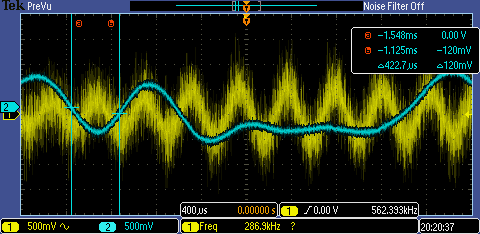
\includegraphics[width=0.65\textwidth]{img/2PAM_SCR.png}
    \caption{2-PAM SCR}
  \end{center}
\end{figure}

\pagebreak
\textbf{Code:}

\begin{verbatim}
	if (counter == 0) {
		symbol = SSRG_update(&SSRG_state); // pseudo random m-sequence
		x[0] = data[symbol]; // read the table

		/* dotting sequence
		symbol = symbol ^ 1;
		x[0] = data[symbol]; // read the table
		*/
	}

	// perform impulse modulation based on the FIR filter, B[N] 

	y  = 0;

	for (i = 0; i < 8; i++) {
		y +=  x[i]*B[counter + 20*i];	// perform the dot-product
	}

	if (counter == (samplesPerSymbol - 1)) {
		counter = -1; 

		/* shift x[] in preparation for the next symbol */

		for (i = 9; i > 0; i--) {
			x[i] = x[i - 1];          // setup x[] for the next input
		}
	}

	counter++;

	output = y;
	scr = clock_recover(y);
\end{verbatim}

\textbf{Table:}

\begin{center}
\begin{tabular}{c|c|c}
pattern	&	frequency & amplitude \\ \hline
dotted sequence	&	 2381 Hz	&	1.04 V				\\ \hline
dotted sequence	&	 2323 Hz	&	1.46 V
\end{tabular}
\end{center}

\textbf{LPF:}

\begin{center}
\begin{tabular}{c|c}
b0	&	 1				\\ \hline
b1	&  1				\\ \hline
b2	&  0				\\ \hline
-a1	&	 0.509525\\ \hline
-a2	&	 0
\end{tabular}
\end{center}

\textbf{Code:}

\begin{verbatim}
  if (counter == 0) {
		symbol = SSRG_update(&SSRG_state); // a faster version of rand() % 2
		x[0] = data[symbol]; // read the table
	}

  // perform impulse modulation based on the FIR filter, B[N] 
  y  = 0;

  for (i = 0; i < 8; i++) {
		y +=  x[i]*B[counter + 20*i];	// perform the dot-product
	}

  if (counter == (samplesPerSymbol - 1)) {
    counter = -1; 

		/* shift x[] in preparation for the next symbol */
 		for (i = 9; i > 0; i--) {
			x[i] = x[i - 1];          // setup x[] for the next input
		}
  }

  counter++;

	output = y*cosine[counter & 3];

	//receiver
	demod = 2*output*cosine[counter & 3];

	//LPF
	biquad_x[0][0] = demod;

	CodecDataOut.Channel[LEFT]  = y; // setup the LEFT  value
	CodecDataOut.Channel[RIGHT] = G[0] * biquad(0, biquad_x[0][0]); // setup the RIGHT value
\end{verbatim}

\begin{figure}[h]
  \begin{center}
    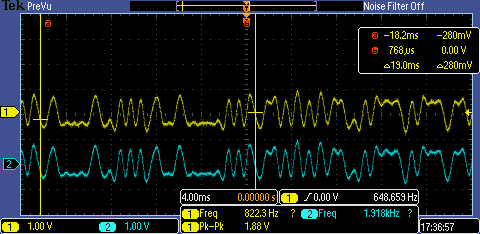
\includegraphics[width=0.65\textwidth]{img/tx_rx.png}
    \caption{Demodulated PAM}
  \end{center}
\end{figure}

\begin{figure}[h]
  \begin{center}
    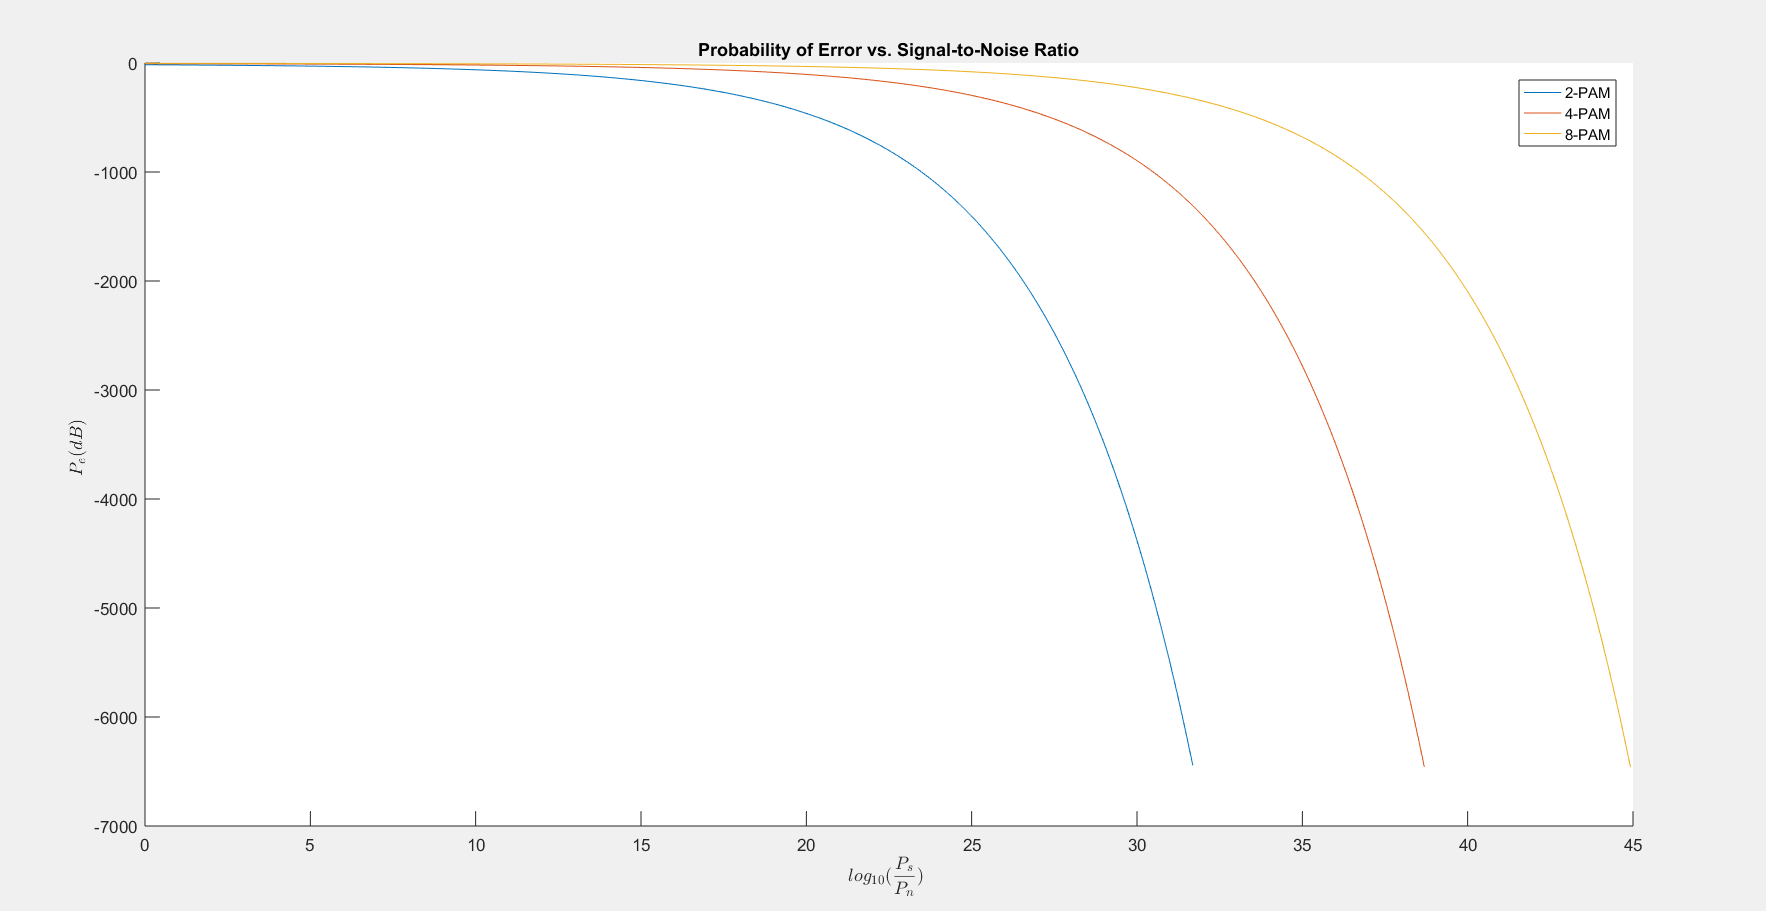
\includegraphics[width=0.65\textwidth]{img/probability_of_error.png}
    \caption{Probability of Error vs. SNR}
  \end{center}
\end{figure}

%----------------------------------------------------------------------------------------
%	SECTION 4
%----------------------------------------------------------------------------------------

\section{Discussion}

\subsection{Pulse Shaping}

When decoding a signal we need to discard the start of a signal.
Pulse shaping with a lot of excess bandwidth allows more room for error in any sampling impairments that are inherent to digital communication.
However, it requires twice as much bandwidth as the ideal nyquist pusle shape.

\subsection{Symbol Clock Recovery (SCR)}

It is clear that for any carrier based communication system it is important for both the transmitter and receiver oscillator to have match frequency and phase.
We observe that both the frequency and phase can be recovered form the received signal.
Before we can recover the frequency and phase the signal needs to be preprocessed.

The preprocessing filters can be implemented using second order sections.
When preprocessing one must be careful to not cause overflows: we had to scale our input and output to avoid this.

\subsection{Demodulation}

Demodulation in the ideal channel is very simple. It is just multiplying by cosine followed by a scaled LPF.
We can implement the LPF with second order sections, so again we need to watch for any error propogation.
Lastly the probability of error vs. SNR is a good theoretical measurement of what you should expect your symbol error rate to be.

%----------------------------------------------------------------------------------------
%	SECTION 5
%----------------------------------------------------------------------------------------

\section{Answers to questions}

\begin{enumerate}
  \begin{item}
		How could pulse shaping be implemented using only a single "filter" (not a bank of filters). Practically, why would this be undesirable?

  \textbf{Answer:}
		Pulse shaping could be implemented by convolving with a single FIR filter. This is undesirable because for baseband transmission we usually take our symbol amplitude vector and upsample (by some fator L) to the DAC frequency before pulse shaping. Because of this upsampling, the amplitude vector contains a lot of extra zeros, which would cause (L - 1) multiplications by 0 for every original symbol amplitude. By using a filter bank, we avoid these
		fruitless multiplications by 0, and obtain a factor of L performance improvement.
  \end{item}

  \begin{item}
		In the clock recovery system, discuss the need for a Prefiltering. For a symbol rate of 2 kHz, what would be the output if the prefilter attenuated all frequencies greater than 900 Hz? Would it be possible to recover the transmitter's symbol frequency (using the same squaring operation and post-filters as in the lab)? If not, give a short reason why.

  \textbf{Answer:}
		We prefilter to obtain a cosine with a center frequency of $fsym/2$ without high frequency noise. What we are interested in is capturing the phase ($\theta$) and frequency information (fsym) of the cosine to feed this into a Costas or Phase Lock Loop to determine the phase offset for sampling. Any other frequency content is unnecessary.

		If the output of the prefilter attenuated all frequencies greater than 900 Hz, we would not be able to recover the transmitter's symbol frequency because $fsym/2$ in this case equals 1 KHz, which would be attenuated by our hypothetical prefilter.
  \end{item}

\end{enumerate}

\end{document}
